% Options for packages loaded elsewhere
\PassOptionsToPackage{unicode}{hyperref}
\PassOptionsToPackage{hyphens}{url}
%
\documentclass[
]{article}
\usepackage{amsmath,amssymb}
\usepackage{lmodern}
\usepackage{iftex}
\ifPDFTeX
  \usepackage[T1]{fontenc}
  \usepackage[utf8]{inputenc}
  \usepackage{textcomp} % provide euro and other symbols
\else % if luatex or xetex
  \usepackage{unicode-math}
  \defaultfontfeatures{Scale=MatchLowercase}
  \defaultfontfeatures[\rmfamily]{Ligatures=TeX,Scale=1}
\fi
% Use upquote if available, for straight quotes in verbatim environments
\IfFileExists{upquote.sty}{\usepackage{upquote}}{}
\IfFileExists{microtype.sty}{% use microtype if available
  \usepackage[]{microtype}
  \UseMicrotypeSet[protrusion]{basicmath} % disable protrusion for tt fonts
}{}
\makeatletter
\@ifundefined{KOMAClassName}{% if non-KOMA class
  \IfFileExists{parskip.sty}{%
    \usepackage{parskip}
  }{% else
    \setlength{\parindent}{0pt}
    \setlength{\parskip}{6pt plus 2pt minus 1pt}}
}{% if KOMA class
  \KOMAoptions{parskip=half}}
\makeatother
\usepackage{xcolor}
\IfFileExists{xurl.sty}{\usepackage{xurl}}{} % add URL line breaks if available
\IfFileExists{bookmark.sty}{\usepackage{bookmark}}{\usepackage{hyperref}}
\hypersetup{
  hidelinks,
  pdfcreator={LaTeX via pandoc}}
\urlstyle{same} % disable monospaced font for URLs
\usepackage{longtable,booktabs,array}
\usepackage{calc} % for calculating minipage widths
% Correct order of tables after \paragraph or \subparagraph
\usepackage{etoolbox}
\makeatletter
\patchcmd\longtable{\par}{\if@noskipsec\mbox{}\fi\par}{}{}
\makeatother
% Allow footnotes in longtable head/foot
\IfFileExists{footnotehyper.sty}{\usepackage{footnotehyper}}{\usepackage{footnote}}
\makesavenoteenv{longtable}
\usepackage{graphicx}
\makeatletter
\def\maxwidth{\ifdim\Gin@nat@width>\linewidth\linewidth\else\Gin@nat@width\fi}
\def\maxheight{\ifdim\Gin@nat@height>\textheight\textheight\else\Gin@nat@height\fi}
\makeatother
% Scale images if necessary, so that they will not overflow the page
% margins by default, and it is still possible to overwrite the defaults
% using explicit options in \includegraphics[width, height, ...]{}
\setkeys{Gin}{width=\maxwidth,height=\maxheight,keepaspectratio}
% Set default figure placement to htbp
\makeatletter
\def\fps@figure{htbp}
\makeatother
\setlength{\emergencystretch}{3em} % prevent overfull lines
\providecommand{\tightlist}{%
  \setlength{\itemsep}{0pt}\setlength{\parskip}{0pt}}
\setcounter{secnumdepth}{-\maxdimen} % remove section numbering
\ifLuaTeX
  \usepackage{selnolig}  % disable illegal ligatures
\fi

\author{}
\date{}

\begin{document}

\hypertarget{cahier-de-conception}{%
\section{CAHIER DE CONCEPTION}\label{cahier-de-conception}}

\hypertarget{chapitre-1-introduction}{%
\section{CHAPITRE 1 : INTRODUCTION}\label{chapitre-1-introduction}}

\hypertarget{contexte}{%
\subsection{1.1 Contexte}\label{contexte}}

À l'issue de la phase d'analyse, les besoins fonctionnels du système ont
été identifiés, modélisés et validés à travers les cas d'utilisation
ainsi que les diagrammes de séquence système.

La phase de conception constitue l'étape suivante du cycle de
développement logiciel. Elle consiste à définir l'organisation interne
de la solution afin de satisfaire les besoins exprimés lors de
l'analyse.

\hypertarget{objectif-de-la-conception}{%
\subsection{1.2 Objectif de la
Conception}\label{objectif-de-la-conception}}

L'objectif de la conception est de définir les différents composants du
système ainsi que leurs interactions.

Cette phase vise notamment à :

\begin{itemize}
\item
  \begin{quote}
  définir l'architecture du système ;
  \end{quote}
\item
  \begin{quote}
  identifier les différents modules de l'application ;
  \end{quote}
\item
  \begin{quote}
  détailler les interactions internes entre les composants ;
  \end{quote}
\item
  \begin{quote}
  élaborer les diagrammes de séquence de conception ;
  \end{quote}
\item
  \begin{quote}
  construire le diagramme de classes ;
  \end{quote}
\item
  \begin{quote}
  préparer l'implémentation de la solution.
  \end{quote}
\end{itemize}

\hypertarget{duxe9marche-adoptuxe9e}{%
\subsection{1.3 Démarche Adoptée}\label{duxe9marche-adoptuxe9e}}

La conception est réalisée selon une approche orientée objet basée sur
UML.

Contrairement à la phase d'analyse où le système est considéré comme une
boîte noire, la conception consiste à décomposer le système en plusieurs
composants collaborant entre eux afin de réaliser les fonctionnalités
attendues.

Les modèles UML utilisés dans cette phase sont :

\begin{itemize}
\item
  \begin{quote}
  le diagramme d'architecture ;
  \end{quote}
\item
  \begin{quote}
  le diagramme de paquetages ;
  \end{quote}
\item
  \begin{quote}
  les diagrammes de séquence de conception ;
  \end{quote}
\item
  \begin{quote}
  le diagramme de classes.
  \end{quote}
\end{itemize}

\hypertarget{chapitre-2-choix-de-larchitecture}{%
\section{CHAPITRE 2 : CHOIX DE
L'ARCHITECTURE}\label{chapitre-2-choix-de-larchitecture}}

\hypertarget{introduction}{%
\subsection{2.1 Introduction}\label{introduction}}

L'architecture logicielle décrit l'organisation générale du système
ainsi que les interactions entre ses principaux composants.

Le choix d'une architecture adaptée facilite la maintenance, l'évolution
et la réutilisation des différents modules de l'application.

\hypertarget{architecture-retenue}{%
\subsection{2.2 Architecture Retenue}\label{architecture-retenue}}

Pour l'application de gestion agricole intelligente, une architecture en
trois couches a été retenue.

Cette architecture permet de séparer les responsabilités du système en
plusieurs niveaux distincts afin de faciliter son développement et sa
maintenance.

Les trois couches retenues sont :

\hypertarget{couche-pruxe9sentation}{%
\subsubsection{Couche Présentation}\label{couche-pruxe9sentation}}

La couche présentation assure les interactions entre les utilisateurs et
le système.

Elle regroupe les interfaces permettant :

\begin{itemize}
\item
  \begin{quote}
  l'authentification ;
  \end{quote}
\item
  \begin{quote}
  la gestion des cultures ;
  \end{quote}
\item
  \begin{quote}
  le suivi des cultures ;
  \end{quote}
\item
  \begin{quote}
  la consultation des prédictions ;
  \end{quote}
\item
  \begin{quote}
  la consultation des recommandations ;
  \end{quote}
\item
  \begin{quote}
  l'administration du système.
  \end{quote}
\end{itemize}

\hypertarget{couche-muxe9tier}{%
\subsubsection{Couche Métier}\label{couche-muxe9tier}}

La couche métier contient les traitements et les règles de gestion de
l'application.

Elle assure notamment :

\begin{itemize}
\item
  \begin{quote}
  la gestion des cultures ;
  \end{quote}
\item
  \begin{quote}
  le suivi des cultures ;
  \end{quote}
\item
  \begin{quote}
  la génération des recommandations ;
  \end{quote}
\item
  \begin{quote}
  la gestion des utilisateurs ;
  \end{quote}
\item
  \begin{quote}
  la coordination des prédictions de rendement.
  \end{quote}
\end{itemize}

\hypertarget{couche-donnuxe9es}{%
\subsubsection{Couche Données}\label{couche-donnuxe9es}}

La couche données assure la persistance des informations manipulées par
le système.

Elle permet notamment le stockage :

\begin{itemize}
\item
  \begin{quote}
  des utilisateurs ;
  \end{quote}
\item
  \begin{quote}
  des cultures ;
  \end{quote}
\item
  \begin{quote}
  des observations ;
  \end{quote}
\item
  \begin{quote}
  des prédictions ;
  \end{quote}
\item
  \begin{quote}
  des recommandations.
  \end{quote}
\end{itemize}

\hypertarget{principe-de-fonctionnement}{%
\subsection{2.3 Principe de
Fonctionnement}\label{principe-de-fonctionnement}}

Le fonctionnement général de l'architecture est le suivant :

\begin{enumerate}
\def\labelenumi{\arabic{enumi}.}
\item
  \begin{quote}
  L'utilisateur interagit avec la couche présentation.
  \end{quote}
\item
  \begin{quote}
  La couche présentation transmet les demandes à la couche métier.
  \end{quote}
\item
  \begin{quote}
  La couche métier applique les règles de gestion nécessaires.
  \end{quote}
\item
  \begin{quote}
  La couche métier sollicite la couche données pour accéder aux
  informations.
  \end{quote}
\item
  \begin{quote}
  Les résultats sont retournés à la couche présentation puis à
  l'utilisateur.
  \end{quote}
\end{enumerate}

Cette organisation permet de réduire le couplage entre les différentes
parties du système et d'améliorer la maintenabilité de l'application.

\hypertarget{chapitre-3-diagramme-de-paquetages}{%
\section{CHAPITRE 3 : DIAGRAMME DE
PAQUETAGES}\label{chapitre-3-diagramme-de-paquetages}}

\hypertarget{introduction-1}{%
\subsection{3.1 Introduction}\label{introduction-1}}

Le diagramme de paquetages permet d'organiser les différents éléments du
système en groupes logiques appelés paquetages.

Chaque paquetage regroupe des éléments ayant des responsabilités
similaires. Cette organisation facilite la compréhension du système et
réduit les dépendances entre les différents modules.

Dans le cadre de cette étude, les paquetages sont définis conformément à
l'architecture en trois couches retenue précédemment.

\hypertarget{identification-des-paquetages}{%
\subsection{3.2 Identification des
Paquetages}\label{identification-des-paquetages}}

Afin de respecter l'architecture en trois couches retenue, le système
est organisé en trois paquetages principaux.

\hypertarget{paquetage-pruxe9sentation}{%
\subsubsection{Paquetage Présentation}\label{paquetage-pruxe9sentation}}

Ce paquetage regroupe les interfaces permettant les interactions entre
les utilisateurs et le système.

Les principaux éléments de ce paquetage sont :

\begin{itemize}
\item
  \begin{quote}
  PageConnexion ;
  \end{quote}
\item
  \begin{quote}
  PageCultures ;
  \end{quote}
\item
  \begin{quote}
  PageSuiviCultures ;
  \end{quote}
\item
  \begin{quote}
  PagePredictions ;
  \end{quote}
\item
  \begin{quote}
  PageRecommandations ;
  \end{quote}
\item
  \begin{quote}
  PageAdministration.
  \end{quote}
\end{itemize}

\hypertarget{paquetage-muxe9tier}{%
\subsubsection{Paquetage Métier}\label{paquetage-muxe9tier}}

Ce paquetage contient les traitements et les règles de gestion de
l'application.

Les principaux éléments de ce paquetage sont :

\begin{itemize}
\item
  \begin{quote}
  GestionAuthentification ;
  \end{quote}
\item
  \begin{quote}
  GestionCultures ;
  \end{quote}
\item
  \begin{quote}
  GestionSuiviCultures ;
  \end{quote}
\item
  \begin{quote}
  GestionPredictions ;
  \end{quote}
\item
  \begin{quote}
  GestionRecommandations ;
  \end{quote}
\item
  \begin{quote}
  GestionUtilisateurs.
  \end{quote}
\end{itemize}

\hypertarget{paquetage-donnuxe9es}{%
\subsubsection{Paquetage Données}\label{paquetage-donnuxe9es}}

Ce paquetage assure la persistance des informations manipulées par le
système.

Les principaux éléments de ce paquetage sont :

\begin{itemize}
\item
  \begin{quote}
  Utilisateur ;
  \end{quote}
\item
  \begin{quote}
  Culture ;
  \end{quote}
\item
  \begin{quote}
  Observation ;
  \end{quote}
\item
  \begin{quote}
  Prediction ;
  \end{quote}
\item
  \begin{quote}
  Recommandation.
  \end{quote}
\end{itemize}

\hypertarget{services-externes}{%
\subsubsection{Services Externes}\label{services-externes}}

\begin{itemize}
\item
  \begin{quote}
  ServicePrediction.
  \end{quote}
\end{itemize}

\hypertarget{relations-entre-les-paquetages}{%
\subsection{3.3 Relations entre les
Paquetages}\label{relations-entre-les-paquetages}}

Les dépendances entre les paquetages sont définies comme suit :

\begin{itemize}
\item
  \begin{quote}
  le paquetage Présentation dépend du paquetage Métier ;
  \end{quote}
\item
  \begin{quote}
  le paquetage Métier dépend du paquetage Données ;
  \end{quote}
\item
  \begin{quote}
  le paquetage Présentation n'accède jamais directement au paquetage
  Données.
  \end{quote}
\end{itemize}

Cette organisation permet de respecter la séparation des responsabilités
et de limiter le couplage entre les différents modules du système.

\hypertarget{diagramme-de-paquetages}{%
\subsection{3.4 Diagramme de Paquetages}\label{diagramme-de-paquetages}}

La figure suivante présente l'organisation générale des paquetages du
système.

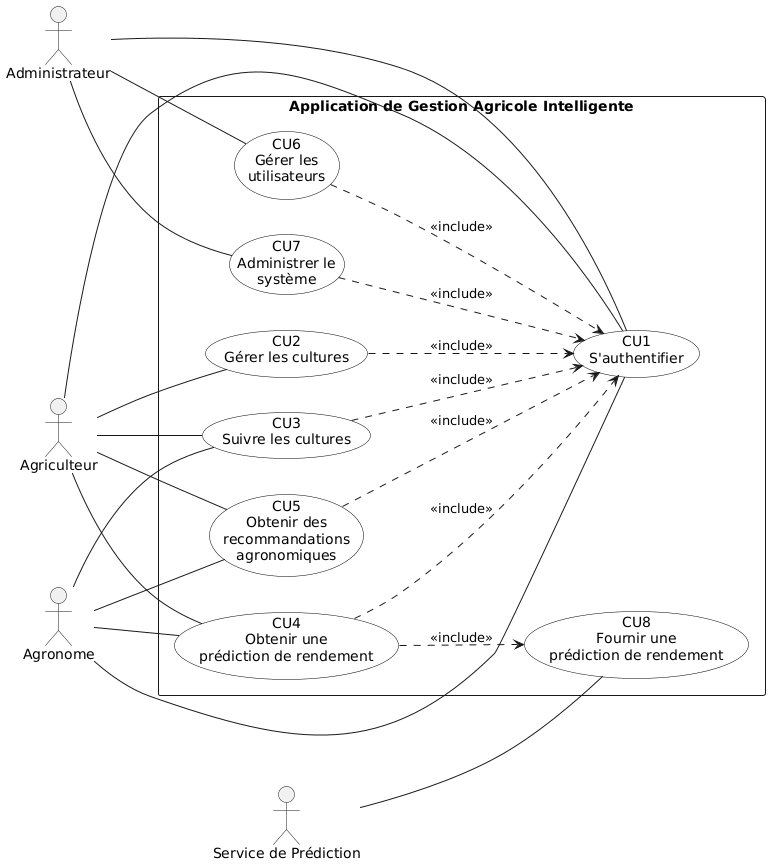
\includegraphics[width=6.69306in,height=2.51111in]{media/image1.png}

\textbf{Figure 3.1 : Diagramme de paquetages de l'application de gestion
agricole intelligente}

\hypertarget{chapitre-4-diagrammes-de-suxe9quence-de-conception}{%
\section{CHAPITRE 4 : DIAGRAMMES DE SÉQUENCE DE
CONCEPTION}\label{chapitre-4-diagrammes-de-suxe9quence-de-conception}}

\hypertarget{introduction-2}{%
\subsection{4.1 Introduction}\label{introduction-2}}

Les diagrammes de séquence de conception permettent de détailler les
interactions internes entre les différents composants du système afin de
réaliser les fonctionnalités identifiées lors de la phase d'analyse.

Contrairement aux diagrammes de séquence système qui considèrent le
système comme une boîte noire, les diagrammes de séquence de conception
mettent en évidence les différents objets impliqués dans le traitement
d'une demande ainsi que les messages échangés entre eux.

Ces diagrammes servent de base à l'identification des classes, des
opérations et des relations qui seront représentées dans le diagramme de
classes.

\hypertarget{diagramme-de-suxe9quence-de-conception-du-cas-dutilisation-cu1-sauthentifier}{%
\subsection{4.2 Diagramme de Séquence de Conception du Cas d'Utilisation
CU1 :
S'authentifier}\label{diagramme-de-suxe9quence-de-conception-du-cas-dutilisation-cu1-sauthentifier}}

Le diagramme suivant présente les interactions entre les différents
composants du système lors du processus d'authentification d'un
utilisateur.

Les objets impliqués sont :

\begin{itemize}
\item
  \begin{quote}
  Agriculteur ;
  \end{quote}
\item
  \begin{quote}
  PageConnexion ;
  \end{quote}
\item
  \begin{quote}
  GestionAuthentification ;
  \end{quote}
\item
  \begin{quote}
  Utilisateur ;
  \end{quote}
\item
  \begin{quote}
  Bd.
  \end{quote}
\end{itemize}

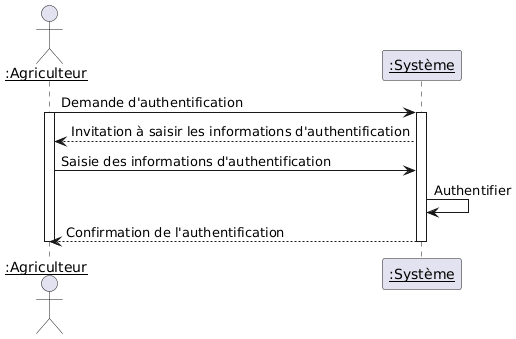
\includegraphics[width=6.69306in,height=3.21944in]{media/image2.png}

\hypertarget{diagramme-de-suxe9quence-de-conception-du-cas-dutilisation-cu2-guxe9rer-les-cultures}{%
\subsection{4.3 Diagramme de Séquence de Conception du Cas d'Utilisation
CU2 : Gérer les
Cultures}\label{diagramme-de-suxe9quence-de-conception-du-cas-dutilisation-cu2-guxe9rer-les-cultures}}

Le diagramme suivant présente les interactions entre les différents
composants du système lors de la gestion des cultures.

Les objets impliqués sont :

\begin{itemize}
\item
  \begin{quote}
  Agriculteur ;
  \end{quote}
\item
  \begin{quote}
  PageCultures ;
  \end{quote}
\item
  \begin{quote}
  GestionCultures ;
  \end{quote}
\item
  \begin{quote}
  Culture ;
  \end{quote}
\item
  \begin{quote}
  Bd.
  \end{quote}
\end{itemize}

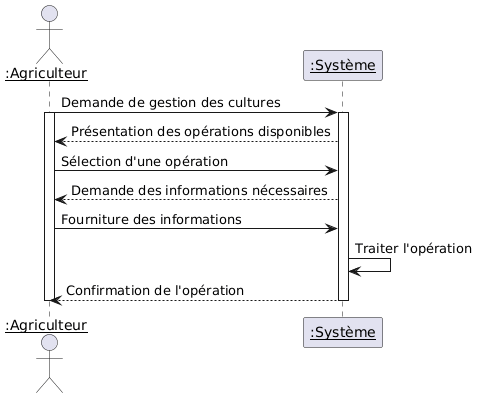
\includegraphics[width=6.69306in,height=3.05903in]{media/image3.png}

\hypertarget{diagramme-de-suxe9quence-de-conception-du-cas-dutilisation-cu3-suivre-les-cultures}{%
\subsection{4.4 Diagramme de Séquence de Conception du Cas d'Utilisation
CU3 : Suivre les
Cultures}\label{diagramme-de-suxe9quence-de-conception-du-cas-dutilisation-cu3-suivre-les-cultures}}

Le diagramme suivant présente les interactions entre les différents
composants du système lors du suivi d'une culture.

Les objets impliqués sont :

\begin{itemize}
\item
  \begin{quote}
  Agriculteur ;
  \end{quote}
\item
  \begin{quote}
  PageSuiviCultures ;
  \end{quote}
\item
  \begin{quote}
  GestionSuiviCultures ;
  \end{quote}
\item
  \begin{quote}
  Observation ;
  \end{quote}
\item
  \begin{quote}
  Culture ;
  \end{quote}
\item
  \begin{quote}
  Bd.
  \end{quote}
\end{itemize}

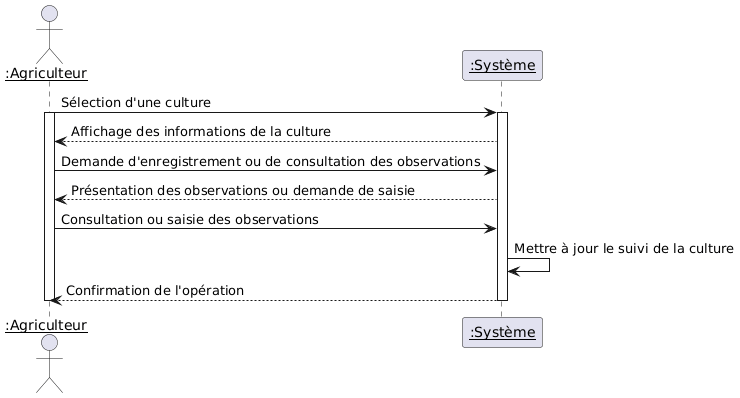
\includegraphics[width=6.69306in,height=3.48681in]{media/image4.png}

\hypertarget{diagramme-de-suxe9quence-de-conception-du-cas-dutilisation-cu4-obtenir-une-pruxe9diction-de-rendement}{%
\subsection{4.5 Diagramme de Séquence de Conception du Cas d'Utilisation
CU4 : Obtenir une Prédiction de
Rendement}\label{diagramme-de-suxe9quence-de-conception-du-cas-dutilisation-cu4-obtenir-une-pruxe9diction-de-rendement}}

Le diagramme suivant présente les interactions entre les différents
composants du système lors de l'obtention d'une prédiction de rendement.

Les objets impliqués sont :

\begin{itemize}
\item
  \begin{quote}
  Agriculteur ;
  \end{quote}
\item
  \begin{quote}
  PagePredictions ;
  \end{quote}
\item
  \begin{quote}
  GestionPredictions ;
  \end{quote}
\item
  \begin{quote}
  Culture ;
  \end{quote}
\item
  \begin{quote}
  ServicePrediction ;
  \end{quote}
\item
  \begin{quote}
  Prediction ;
  \end{quote}
\item
  \begin{quote}
  Bd.
  \end{quote}
\end{itemize}

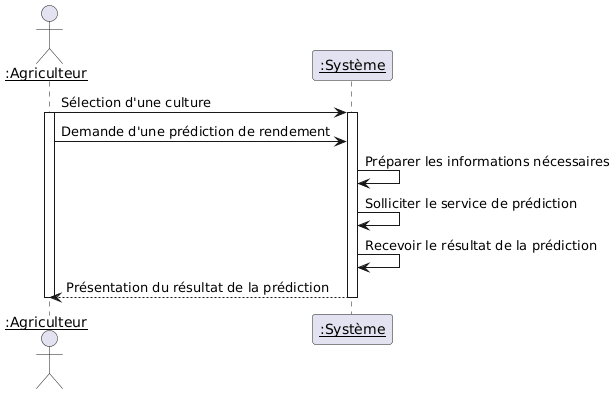
\includegraphics[width=6.69306in,height=3.34028in]{media/image5.png}

\hypertarget{diagramme-de-suxe9quence-de-conception-du-cas-dutilisation-cu5-obtenir-des-recommandations-agronomiques}{%
\subsection{4.6 Diagramme de Séquence de Conception du Cas d'Utilisation
CU5 : Obtenir des Recommandations
Agronomiques}\label{diagramme-de-suxe9quence-de-conception-du-cas-dutilisation-cu5-obtenir-des-recommandations-agronomiques}}

Le diagramme suivant présente les interactions entre les différents
composants du système lors de l'obtention de recommandations
agronomiques.

Les objets impliqués sont :

\begin{itemize}
\item
  \begin{quote}
  Agriculteur ;
  \end{quote}
\item
  \begin{quote}
  PageRecommandations ;
  \end{quote}
\item
  \begin{quote}
  GestionRecommandations ;
  \end{quote}
\item
  \begin{quote}
  Culture ;
  \end{quote}
\item
  \begin{quote}
  Recommandation ;
  \end{quote}
\item
  \begin{quote}
  Bd.
  \end{quote}
\end{itemize}

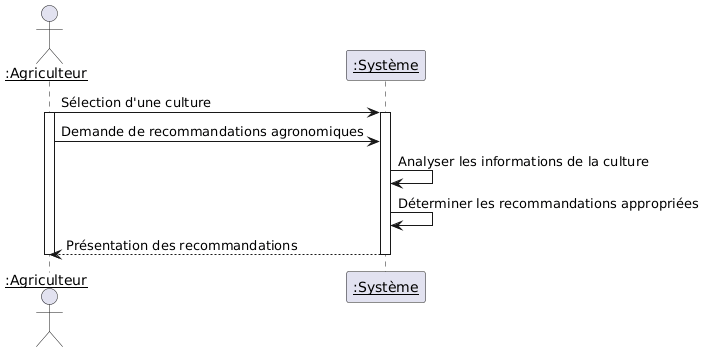
\includegraphics[width=6.69306in,height=3.04792in]{media/image6.png}

\hypertarget{diagramme-de-suxe9quence-de-conception-du-cas-dutilisation-cu6-guxe9rer-les-utilisateurs}{%
\subsection{4.7 Diagramme de Séquence de Conception du Cas d'Utilisation
CU6 : Gérer les
Utilisateurs}\label{diagramme-de-suxe9quence-de-conception-du-cas-dutilisation-cu6-guxe9rer-les-utilisateurs}}

Le diagramme suivant présente les interactions entre les différents
composants du système lors de la gestion des utilisateurs.

Les objets impliqués sont :

\begin{itemize}
\item
  \begin{quote}
  Administrateur ;
  \end{quote}
\item
  \begin{quote}
  PageAdministration ;
  \end{quote}
\item
  \begin{quote}
  GestionUtilisateurs ;
  \end{quote}
\item
  \begin{quote}
  Utilisateur ;
  \end{quote}
\item
  \begin{quote}
  Bd.
  \end{quote}
\end{itemize}

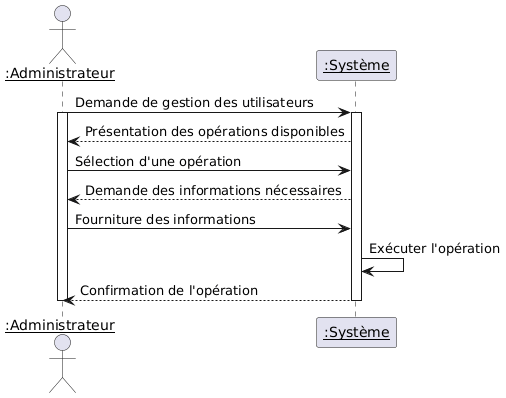
\includegraphics[width=6.69306in,height=2.99583in]{media/image7.png}

\hypertarget{diagramme-de-suxe9quence-de-conception-du-cas-dutilisation-cu7-administrer-le-systuxe8me}{%
\subsection{4.8 Diagramme de Séquence de Conception du Cas d'Utilisation
CU7 : Administrer le
Système}\label{diagramme-de-suxe9quence-de-conception-du-cas-dutilisation-cu7-administrer-le-systuxe8me}}

Le diagramme suivant présente les interactions entre les différents
composants du système lors des opérations d'administration.

Les objets impliqués sont :

\begin{itemize}
\item
  \begin{quote}
  Administrateur ;
  \end{quote}
\item
  \begin{quote}
  PageAdministration ;
  \end{quote}
\item
  \begin{quote}
  GestionUtilisateurs ;
  \end{quote}
\item
  \begin{quote}
  Bd.
  \end{quote}
\end{itemize}

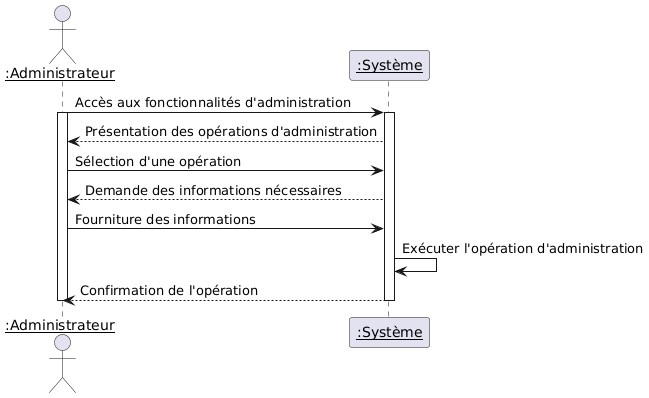
\includegraphics[width=6.69306in,height=3.20278in]{media/image8.png}

\hypertarget{chapitre-5-diagramme-de-classes}{%
\section{CHAPITRE 5 : DIAGRAMME DE
CLASSES}\label{chapitre-5-diagramme-de-classes}}

\hypertarget{introduction-3}{%
\subsection{5.1 Introduction}\label{introduction-3}}

Le diagramme de classes constitue l'un des principaux modèles de la
conception orientée objet.

Il permet de représenter la structure statique du système en identifiant
les différentes classes, leurs attributs, leurs opérations ainsi que les
relations qui les unissent.

Les classes présentées dans ce chapitre ont été identifiées à partir des
diagrammes de séquence de conception élaborés précédemment.

Le diagramme de classes servira également de base à la conception de la
base de données ainsi qu'à l'implémentation de l'application.

\hypertarget{diagramme-de-classes}{%
\subsection{5.2 Diagramme de Classes}\label{diagramme-de-classes}}

\includegraphics[width=5.49444in,height=5.41806in]{media/image9.png}Le
diagramme de classes suivant représente la structure statique de
l'application de gestion agricole intelligente.

Il met en évidence les différentes classes métier identifiées lors de la
phase de conception, leurs attributs, leurs opérations ainsi que les
relations existantes entre elles.

Le diagramme constitue la base de la conception de la base de données et
de l'implémentation de l'application.

\hypertarget{chapitre-6-moduxe8le-de-donnuxe9es}{%
\section{CHAPITRE 6 : MODÈLE DE
DONNÉES}\label{chapitre-6-moduxe8le-de-donnuxe9es}}

\hypertarget{introduction-4}{%
\subsection{6.1 Introduction}\label{introduction-4}}

Le modèle de données constitue la traduction du diagramme de classes
vers un modèle relationnel exploitable par un système de gestion de base
de données.

Il permet de définir les différentes tables nécessaires au stockage des
informations ainsi que les relations existantes entre elles.

Le modèle présenté dans ce chapitre est directement dérivé du diagramme
de classes élaboré lors de la phase de conception.

\hypertarget{passage-du-diagramme-de-classes-au-moduxe8le-relationnel}{%
\subsection{6.2 Passage du Diagramme de Classes au Modèle
Relationnel}\label{passage-du-diagramme-de-classes-au-moduxe8le-relationnel}}

Le passage du diagramme de classes au modèle relationnel repose sur les
règles suivantes :

\begin{itemize}
\item
  \begin{quote}
  chaque classe persistante devient une table ;
  \end{quote}
\item
  \begin{quote}
  chaque attribut devient un champ de la table correspondante ;
  \end{quote}
\item
  \begin{quote}
  les relations entre classes sont traduites par des clés étrangères ;
  \end{quote}
\item
  \begin{quote}
  les relations d'héritage sont matérialisées par des tables
  spécialisées liées à leur classe mère.
  \end{quote}
\end{itemize}

Le modèle relationnel obtenu permet de conserver la structure définie
lors de la conception orientée objet.

\hypertarget{description-des-tables}{%
\subsection{6.3 Description des Tables}\label{description-des-tables}}

\hypertarget{table-utilisateur}{%
\subsubsection{Table UTILISATEUR}\label{table-utilisateur}}

\begin{longtable}[]{@{}lll@{}}
\toprule
\endhead
Champ & Type & Description \\
idUtilisateur & INT & Identifiant de l'utilisateur \\
nom & VARCHAR & Nom de l'utilisateur \\
prenom & VARCHAR & Prénom de l'utilisateur \\
email & VARCHAR & Adresse électronique \\
motDePasse & VARCHAR & Mot de passe \\
\bottomrule
\end{longtable}

\hypertarget{table-agriculteur}{%
\subsubsection{Table AGRICULTEUR}\label{table-agriculteur}}

\begin{longtable}[]{@{}lll@{}}
\toprule
\endhead
Champ & Type & Description \\
idAgriculteur & INT & Identifiant de l'agriculteur \\
idUtilisateur & INT & Référence vers UTILISATEUR \\
\bottomrule
\end{longtable}

\hypertarget{table-agronome}{%
\subsubsection{Table AGRONOME}\label{table-agronome}}

\begin{longtable}[]{@{}lll@{}}
\toprule
\endhead
Champ & Type & Description \\
idAgronome & INT & Identifiant de l'agronome \\
idUtilisateur & INT & Référence vers UTILISATEUR \\
\bottomrule
\end{longtable}

\hypertarget{table-administrateur}{%
\subsubsection{Table ADMINISTRATEUR}\label{table-administrateur}}

\begin{longtable}[]{@{}lll@{}}
\toprule
\endhead
Champ & Type & Description \\
idAdministrateur & INT & Identifiant de l'administrateur \\
idUtilisateur & INT & Référence vers UTILISATEUR \\
\bottomrule
\end{longtable}

\hypertarget{table-culture}{%
\subsubsection{Table CULTURE}\label{table-culture}}

\begin{longtable}[]{@{}lll@{}}
\toprule
\endhead
Champ & Type & Description \\
idCulture & INT & Identifiant de la culture \\
nomCulture & VARCHAR & Nom de la culture \\
superficie & FLOAT & Superficie cultivée \\
localisation & VARCHAR & Localisation de la culture \\
dateSemis & DATE & Date de semis \\
statut & VARCHAR & État actuel de la culture \\
idAgriculteur & INT & Référence vers AGRICULTEUR \\
\bottomrule
\end{longtable}

\hypertarget{table-observation}{%
\subsubsection{Table OBSERVATION}\label{table-observation}}

\begin{longtable}[]{@{}lll@{}}
\toprule
\endhead
Champ & Type & Description \\
idObservation & INT & Identifiant de l'observation \\
dateObservation & DATE & Date d'observation \\
description & TEXT & Description de l'observation \\
idCulture & INT & Référence vers CULTURE \\
\bottomrule
\end{longtable}

\hypertarget{table-prediction}{%
\subsubsection{Table PREDICTION}\label{table-prediction}}

\begin{longtable}[]{@{}lll@{}}
\toprule
\endhead
Champ & Type & Description \\
idPrediction & INT & Identifiant de la prédiction \\
datePrediction & DATE & Date de la prédiction \\
rendementEstime & FLOAT & Rendement estimé \\
niveauConfiance & FLOAT & Niveau de confiance \\
idCulture & INT & Référence vers CULTURE \\
\bottomrule
\end{longtable}

\hypertarget{table-recommandation}{%
\subsection{Table RECOMMANDATION}\label{table-recommandation}}

\begin{longtable}[]{@{}lll@{}}
\toprule
\endhead
Champ & Type & Description \\
idRecommandation & INT & Clé primaire \\
dateRecommandation & DATE & Date de génération \\
type & VARCHAR(100) & Type de recommandation \\
contenu & TEXT & Contenu détaillé \\
idCulture & INT & Clé étrangère vers CULTURE \\
\bottomrule
\end{longtable}

\hypertarget{schuxe9ma-relationnel-global}{%
\section{6.4 Schéma Relationnel
Global}\label{schuxe9ma-relationnel-global}}

Le schéma relationnel global de la base de données est présenté
ci-dessous :

UTILISATEUR(

idUtilisateur,

nom,

prenom,

email,

motDePasse

)

AGRICULTEUR(

idAgriculteur,

idUtilisateur

)

AGRONOME(

idAgronome,

idUtilisateur

)

ADMINISTRATEUR(

idAdministrateur,

idUtilisateur

)

CULTURE(

idCulture,

nomCulture,

superficie,

localisation,

dateSemis,

statut,

idAgriculteur

)

OBSERVATION(

idObservation,

dateObservation,

description,

idCulture

)

PREDICTION(

idPrediction,

datePrediction,

rendementEstime,

niveauConfiance,

idCulture

)

RECOMMANDATION(

idRecommandation,

dateRecommandation,

type,

contenu,

idCulture

)

\hypertarget{diagramme-relationnel-de-la-base-de-donnuxe9es}{%
\subsection{6.5 Diagramme Relationnel de la Base de
Données}\label{diagramme-relationnel-de-la-base-de-donnuxe9es}}

Le diagramme relationnel suivant présente l'organisation des tables de
la base de données ainsi que les relations établies entre elles.

Il met en évidence les clés primaires, les clés étrangères et les
associations résultant de la transformation du diagramme de classes vers
le modèle relationnel.

\includegraphics[width=6.69306in,height=5.07361in]{media/image10.png}

Ce diagramme constitue la représentation logique de la base de données
qui sera utilisée lors de l'implémentation de l'application.

\hypertarget{chapitre-7-conclusion}{%
\section{CHAPITRE 7 : CONCLUSION}\label{chapitre-7-conclusion}}

La phase de conception a permis de définir l'organisation interne de
l'application de gestion agricole intelligente à partir des besoins
identifiés lors de la phase d'analyse.

Cette étape a conduit au choix d'une architecture en trois couches
composée de la couche présentation, de la couche métier et de la couche
données. Cette architecture favorise la séparation des responsabilités
et facilite la maintenance ainsi que l'évolution future du système.

Les différents composants de l'application ont été structurés à travers
un diagramme de paquetages permettant d'organiser les fonctionnalités
selon leurs rôles respectifs. Les diagrammes de séquence de conception
ont ensuite permis de détailler les interactions internes entre les
différents composants du système pour la réalisation des principaux cas
d'utilisation.

L'identification des classes métier et de leurs relations a conduit à
l'élaboration du diagramme de classes, véritable représentation statique
de la solution. Ce modèle a ensuite servi de base à la conception du
modèle relationnel et à la définition de la structure de la base de
données.

Le modèle obtenu assure une cohérence complète entre les besoins
exprimés dans le cahier des charges, les modèles d'analyse, les modèles
de conception et la future implémentation du système.

La conception réalisée constitue ainsi un guide de référence pour le
développement de l'application. Les différents modèles produits
permettront de faciliter l'implémentation des fonctionnalités de gestion
des cultures, de suivi agricole, de prédiction des rendements et de
recommandation agronomique tout en garantissant la qualité et la
maintenabilité de la solution logicielle.

\end{document}
